\begin{enumerate}[font=\bfseries]

    \item \textbf{For the image below (let’s call it image A), apply a 3x3
    averaging low pass filter and call it image B. Apply the same averaging
    filter to Image B to produce image C.  Draw image B and C. Explain what
    happens when you repeatedly apply an averaging filter to an image?}

    % Make script to generate image and apply filter.
    
    I made a script to apply the averaging filter:

    \begin{figure}[H]
	\centering
	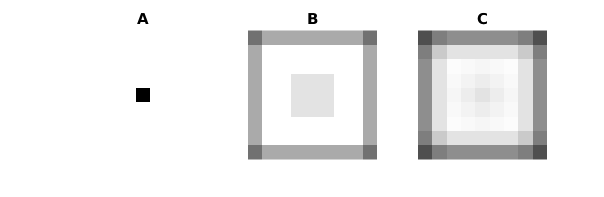
\includegraphics[scale=0.75]{q1.png}
	\caption{Consecutive 3x3 Average Filter}
    \end{figure}

    First I will comment on the dark border that appears, this comes up because
    I used zero padding, and as this was only a 9x9 image, it made a significant
    impact on the image.

    As for the original image contents, as we perform the averaging filter the
    single pixel in the center seems to disperse. If we were to continue
    applying this filter, the dot would disappear and then the image would
    completely turn black dues to the zero padding.

    \item \textbf{In Image shown here, each bar has a width of 6 pixels. The
    gaps between bars are 19 pixels. Explain the result of filtering this image
    using an averaging mask of 25x25 and 20x20}

    % Make script to generate image and apply filter.

    I also made a script to  generate images for this case as well.

    \begin{figure}[H]
	\centering
	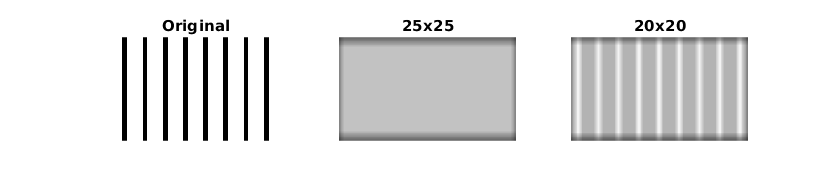
\includegraphics[scale=0.6]{q2.png}
	\caption{25x25 vs. 20x20 Average Filter}
    \end{figure}

    First, there was zero padding and so you can see black seep in from the top
    and bottom of the image.

    The 25x25 filter is "resonant" with the image. Even as we move the filter
    across the image, the value remains the same since 6 + 19 = 25. And so we
    get a completely constant grey as a result. In the case of the 20x20 filter,
    there is a point where there is a vast majority of white pixels, and so we
    get a mostly white pixel as a result. As it moves further it reaches a
    maximum number of black pixels, and will output a constant intensity until
    the black bar leaves he frame. 

    This example starts making me think about how frequency analysis in an image
    could come about, and the affect of filter size on frequency
    characteristics.

    \item \textbf{In spatial filtering, a mask is applied to top-left corner of
    an image and then the center of the mask will be moved through the image. At
    each location, the sum of product of the mask coefficients with the
    corresponding pixel values at that location is calculated. Then the pixel
    value of the image corresponding with the center of the mask will be
    updated. Considering an averaging mask of size $n\times n$with coefficients
    of $\frac{1}{n^2}$.  Calculate the minimum computational complexity of
    applying the averaging filter to an image.  Remember that for an averaging
    mask all the coefficients are one considering a scale factor of
    $\frac{1}{n^2}$.}

    A dot product of a 2 dimensional mask to an image is made up of
    multiplication and addition operations. The operations required are simply
    $n^2$ multiplies and $n^2 - 1$ additions.

    In the case where N is a power of two, multiplication/division operation is
    replaced by a bit shift, which significantly decreases the processing
    requirements.

    \item \textbf{A digital image $f(x,y)$ is  changed to a  black and white
    image $b(x,y)$.  $b(x,y)$ is passed through a 3x3 blurring filter as shown
    here to produce output image $o(x,y)$. What are possible intensity values in
    the output?}

    It important to note that the sum of the coefficients is one. In the case
    where all the pixel values are 255, the output would b 255. When all the
    values are 0, the output is zero. This can be mapped to all values, and so
    the possible values of the output are anywhere from 0 - 255.

\end{enumerate}

\pagebreak

\appendix

\section{Code Listings}

\subsection{Script for Question 1}

\lstinputlisting[style=mattLab]{../q1.m}

\pagebreak

\subsection{Script for Question 2}

\lstinputlisting[style=mattLab]{../q2.m}
